\begin{frame}
	\myheading{Module 18.3: Local Independencies in a Markov Network}
\end{frame}

\begin{frame}
	\begin{columns}
		\column{0.5\textwidth}
		\begin{overlayarea}{\textwidth}{\textheight}
		\end{overlayarea}
		\column{0.5\textwidth}
		\begin{overlayarea}{\textwidth}{\textheight}
			\begin{itemize}[<+->]\justifying
				\item Let $U$ be the set of all random variables in our joint distribution 
				\item Let $X,Y,Z$ be some distinct subsets of $U$
				\item A distribution $P$ over these RVs would imply $X\bot Y|Z$ if and only if we can write 
				\begin{align*}
				P(X) = \phi_1(X,Z)\phi_2(Y,Z)
				\end{align*}
				\item Let us see this in the context of our original example
			\end{itemize}
		\end{overlayarea}
	\end{columns}
\end{frame}

\begin{frame}
	\begin{columns}
		\column{0.5\textwidth}
		\begin{overlayarea}{\textwidth}{\textheight}
			\begin{center}
					\tikzstyle{input_neuron}=[circle,draw=red!50,fill=orange!10,thick]
					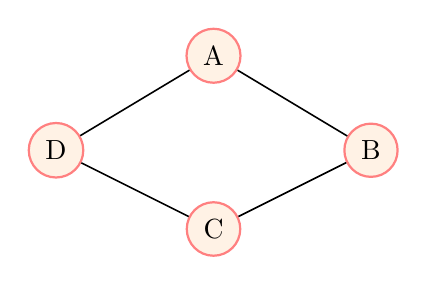
\begin{tikzpicture}
						\node [input_neuron](input0) at (5.5,-0.1)  {D};
						\node [input_neuron] (input1) at (9.5,-0.1)  {B};
						\node [input_neuron] (input2) at (7.5, 1.1) {A};
						\node [input_neuron] (input3) at (7.5, -1.1) {C};
						
						\draw [line width=0.2mm, -] (input0) -- (input2);
						\draw [line width=0.2mm, -] (input0) -- (input3);
						\draw [line width=0.2mm, -] (input1) -- (input2);
						\draw [line width=0.2mm, -] (input1) -- (input3);
					\end{tikzpicture}
				\end{center}

		\end{overlayarea}
		\column{0.5\textwidth}
		\begin{overlayarea}{\textwidth}{\textheight}
			\begin{itemize}[<+->]\justifying
				\item In this example
				\begin{align*}
					&P(A,B,C,D) =\\
					&\frac{1}{Z} [ \phi_1(A,B) \phi_2(B,C) \phi_3(C,D) \phi_4(D,A)]
				\end{align*}
				\item We can rewrite this as 
				\begin{align*}
					&P(A,B,C,D) =\\
					&\frac{1}{Z} \underbrace{[ \phi_1(A,B) \phi_2(B,C) ]}_{\phi_5(B,\{A,C\})} \underbrace{[\phi_3(C,D) \phi_4(D,A)]}_{\phi_6(D,\{A,C\})}
				\end{align*}
				\item We can say that $B \bot D|\{A,C\}$ which is indeed true
			\end{itemize}
		\end{overlayarea}
	\end{columns}
\end{frame}

\begin{frame}
	\begin{columns}
		\column{0.5\textwidth}
		\begin{overlayarea}{\textwidth}{\textheight}
			\begin{center}
					\tikzstyle{input_neuron}=[circle,draw=red!50,fill=orange!10,thick]
					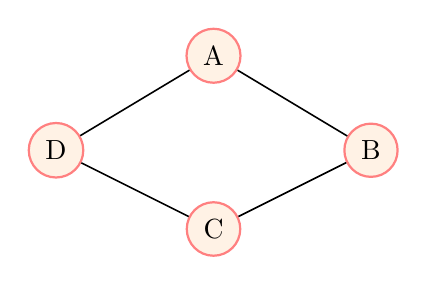
\begin{tikzpicture}
						\node [input_neuron](input0) at (5.5,-0.1)  {D};
						\node [input_neuron] (input1) at (9.5,-0.1)  {B};
						\node [input_neuron] (input2) at (7.5, 1.1) {A};
						\node [input_neuron] (input3) at (7.5, -1.1) {C};
						
						\draw [line width=0.2mm, -] (input0) -- (input2);
						\draw [line width=0.2mm, -] (input0) -- (input3);
						\draw [line width=0.2mm, -] (input1) -- (input2);
						\draw [line width=0.2mm, -] (input1) -- (input3);
					\end{tikzpicture}
				\end{center}
		\end{overlayarea}
		\column{0.5\textwidth}
		\begin{overlayarea}{\textwidth}{\textheight}
			\begin{itemize}[<+->]\justifying
				\item In this example
				\begin{align*}
					&P(A,B,C,D) = \\
					&\frac{1}{Z} [ \phi_1(A,B) \phi_2(B,C) \phi_3(C,D) \phi_4(D,A)]
				\end{align*}
				\item Alternatively we can rewrite this as 
				\begin{align*}
					&P(A,B,C,D) = \\
					&\frac{1}{Z} \underbrace{[ \phi_1(A,B) \phi_2(D,A) ]}_{\phi_5(A,\{B,D\})} \underbrace{[\phi_3(C,D) \phi_4(B,C)]}_{\phi_6(C,\{B,D\})}
				\end{align*}
				\item We can say that $A \bot C|\{B,D\}$ which is indeed true
			\end{itemize}
		\end{overlayarea}
	\end{columns}
\end{frame}

\begin{frame}
	\begin{columns}
		\column{0.5\textwidth}
		\begin{overlayarea}{\textwidth}{\textheight}
			\centering
			\vspace{1cm}\
			\tikzset{mystyle/.style={shape=circle,fill=black,scale=0.3}}
			\tikzset{neigh/.style={shape=circle,fill=blue,scale=0.5}}
			\tikzset{cent/.style={shape=circle,fill=red,scale=0.5}}
			\tikzstyle{input_neuron}=[circle,draw=red!50,fill=orange!10,thick,minimum size=3mm]
			\begin{tikzpicture}[scale=.8]
            % setup the nodes
            \foreach \x in {0,...,5}
            \foreach \y in {0,...,5}
            {
            \ifnum\x=3
                \ifnum\y=2
                    \node[cent] (\x-\y) at (\x,\y){};
                \else
                    \node[mystyle] (\x-\y) at (\x,\y){};
                \fi
            \else
                \node[mystyle] (\x-\y) at (\x,\y){};
            \fi
            }
            % circle selected nodes with letters
            \foreach \mynode/\mytext in {2-2/A,3-3/B,3-1/C,4-2/D}
            {
                \draw[neigh] (\mynode) circle (0.2cm) node {};
            }
			\draw [line width=0.2mm, -] (2.1,2) -- (2.9,2);
			\draw [line width=0.2mm, -] (3,2.9) -- (3,2.1);
			\draw [line width=0.2mm, -] (3,1.1) -- (3,1.9);
			\draw [line width=0.2mm, -] (3.9,2) -- (3.1,2);
	        \end{tikzpicture}
		\end{overlayarea}
		\column{0.5\textwidth}
		\begin{overlayarea}{\textwidth}{\textheight}
			\begin{itemize}[<+->]\justifying
				\item For a given Markov network $H$ we define Markov Blanket of a RV $X$ to be the neighbors of $X$ in $H$
				\item Analogous to the case of Bayesian Networks we can define the local independences associated with $H$ to be
				\begin{align*}
					\color{red} X \color{black} \bot (U - \{X\} - MB_H) | \color{blue}MB_H(X)\color{black}
				\end{align*}  
			\end{itemize}
		\end{overlayarea}
	\end{columns}
\end{frame}

\begin{frame}
	\begin{columns}
		\column{0.5\textwidth}
		\begin{overlayarea}{\textwidth}{0.7\textheight}
			\begin{center}
			Bayesian network
			\end{center}
			\begin{center}
				\tikzstyle{input_neuron}=[ellipse,draw=red!50,fill=orange!10,thick,scale=0.7]
				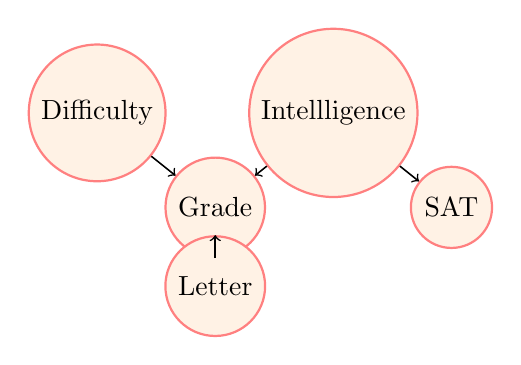
\begin{tikzpicture}
					\node [input_neuron](input0) at (7,-0.1)  {Grade};
					\node [input_neuron] (input1) at (10,-0.1)  {SAT};
					\node [input_neuron] (input2) at (8.5, 1.1) {Intellligence};
					\node [input_neuron] (input3) at (7, -1.1) {Letter};
					\node [input_neuron](input4) at (5.5,1.1)  {Difficulty};

					\draw [line width=0.2mm, ->] (input2) -- (input0);
					\draw [line width=0.2mm, ->] (input0) -- (input3);
					\draw [line width=0.2mm, ->] (input2) -- (input1);
					\draw [line width=0.2mm, ->] (input4) -- (input0);
				\end{tikzpicture}
			\end{center}
	        \vspace{0.4cm}
			Local Independencies 
			\begin{align*}
				X_i \bot NonDescendents_{X_i} | Parent_{X_i}^G
			\end{align*}

		\end{overlayarea}
		\column{0.5\textwidth}
		\begin{overlayarea}{\textwidth}{0.7\textheight}
			\begin{center}
			Markov network\\
			\vspace{0.2cm}
			\tikzset{mystyle/.style={shape=circle,fill=black,scale=0.3}}
			\tikzset{neigh/.style={shape=circle,fill=blue,scale=0.5}}
			\tikzset{cent/.style={shape=circle,fill=red,scale=0.5}}
			\tikzstyle{input_neuron}=[circle,draw=red!50,fill=orange!10,thick,minimum size=3mm]
			\onslide<2->{\begin{tikzpicture}[scale=.6]
            % setup the nodes
            \foreach \x in {0,...,5}
            \foreach \y in {0,...,5}
            {
            \ifnum\x=3
                \ifnum\y=2
                    \node[cent] (\x-\y) at (\x,\y){};
                \else
                    \node[mystyle] (\x-\y) at (\x,\y){};
                \fi
            \else
                \node[mystyle] (\x-\y) at (\x,\y){};
            \fi
            }
            % circle selected nodes with letters
            \foreach \mynode/\mytext in {2-2/A,3-3/B,3-1/C,4-2/D}
            {
                \draw[neigh] (\mynode) circle (0.2cm) node {};
            }
			\draw [line width=0.2mm, -] (2.1,2) -- (2.9,2);
			\draw [line width=0.2mm, -] (3,2.9) -- (3,2.1);
			\draw [line width=0.2mm, -] (3,1.1) -- (3,1.9);
			\draw [line width=0.2mm, -] (3.9,2) -- (3.1,2);
	        \end{tikzpicture}\\}
			\end{center}
	        \vspace{0.4cm}
	        \onslide<3->{Local Independencies 
			\begin{align*}
				X_i \bot NonNeighbors_{X_i} | Neighbors_{X_i}^G
			\end{align*}}
		\end{overlayarea}
	\end{columns}
\end{frame}
